\chapter{The Historical Search System} % (fold)
\label{cha:the_historical_search_system}

To show researchers the qualitative results of the HistDiv algorithm, a search system was developed. The system is also a showcase for the baselines so that results from various algorithms can be compared qualitatively. A seperate system was also developed for evaluators to judge documents from the pools. In this chapter, the architecture and user interface of the historical search system are described in detail.

\section{Architecture} % (fold)
\label{sec:Historical_search}

\subsection{Server side} % (fold)
\label{sub:server_side}

The backend of the Historical Search system comprises of 2 major components: the \textbf{retrieval module} and the \textbf{aspect miner}. The development of both components was carried out in Java. The documents from the NYT corpus were first indexed using the standard Lucene 4.0 API. All fields for all documents were indexed using the standard analyzer.

The aspect miner is responsible for mining topics from the documents. Wikiminer is a REST API that is freely available. A java client was developed for the annotation service so that it can be easily used in the aspect miner. The mined topics with their confidence scores are stored in a Redis database and not in the Lucene index. This is because we only need to lookup the topics for each document when computing diversity. Redis is a high performance key value store that maximizes throughput. The data is stored in JSON which Redis supports natively. The aspect miner component is heavily parallelized and can be used during index creation as well as on demand. 

The main component of the system though is the ranking component housed inside the retrieval module. A REST API using the JAX-RS specification is the interface between frontend and backend. The API has a set of endpoints that cater to different funtionalities of the system. The data exchange format used by the API is JSON. The major endpoint is the \texttt{reRank} endpoint which accepts a HTTP GET request with the following parameters:

\begin{itemize}
	\item q: the query specified by the user
	\item dmin: start date filter
	\item dmax: end date filter
	\item method: the type of retrieval model to use.
	\item k: the number of results
\end{itemize}

\begin{figure}[!h]
\centering
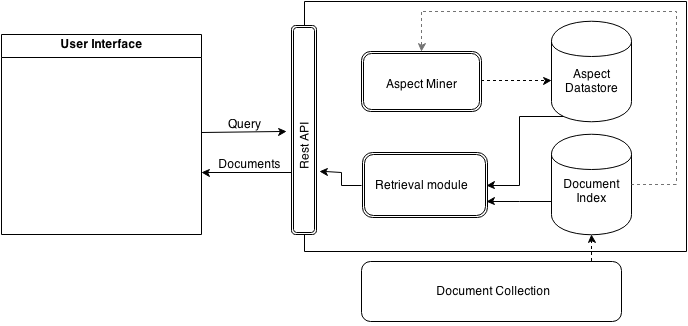
\includegraphics[width=0.9\columnwidth]{images/architecture.png}
\caption{System Architecture}
\label{fig:sysarc}
\end{figure}

The architecture of the system is shown in Figure~\ref{fig:sysarc} where the dashed lines represent processes that have completed before the system went online. Every competitor mentioned in the experiments section is available to the user. The user can also specify a date range to limit his search results. When the reRank endpoint receives a request, it first retrieves the top 1000 documents using the query q and specified date range. If the range is \texttt{null} then the whole 20 year span of the corpus is considered. The results returned from the index are then given as input to the algorithm mention in the method parameter. The algorithm then returns the top k results from the 1000 given as input. The results are returned to the user as a JSON array with all the fields of each document populated. CORS headers are also sent with the result to allow clients running on different servers to use the API as well.

\subsection{Client side} % (fold)
\label{sub:client_side}

The frontend of the Historical Search system is a single page client side application developed using Backbone.js. Backbone.js is a javascript framework for building interactive client side applications that work with data through REST APIs. The UI framework used was Bootstrap 3.0, a responsive framework based purely on CSS and Javascript. The UI itself consists of 3 components: the search bar, the timeline and the search result display. 

The search bar consists of an input text box for the user to enter his query and a selector for the type of diversification algorithm to use. There is also a search button for the user to initiate his search. When the user initiates a search, an AJAX request is made to the reRank endpoint of the rank API with the user's query and method. The date filters are initially set to null. Once the results are returned, the timeline component creates the input JSON data it needs from the returned results. Once the timeline component has initialized, the timeline and search results are rendered on the screen. Highcharts API is used to generate the timeline. The timeline is a bar chart of the number of documents at a given date. Highcharts also has a feature for zooming into tinmelines by highlighting the required area on the timeline. This zooming in triggers another search request to be fired albeit with the date range filter now representing the boundaries of the newly selected portion of the timeline. By clicking on the back arrow of the browser the user can zoom out and return to his previous state. Each bar in the timeline when clicked displays a preview of the article from that date. 

The search results are displayed in a newspaper style format as shown in Figure \ref{fig:ui}. Each document is represented by its headline, publication date and body. News articles which are more relevant to the query according to the ranking method chosen are given more area to display the contents of the body. To neatly present these results of uneven area freewall.js was used. It uses a packing algorithm to reduces the amount of white space between articles, thus giving it the look of a newspaper. 

\begin{figure}[!h]
\centering
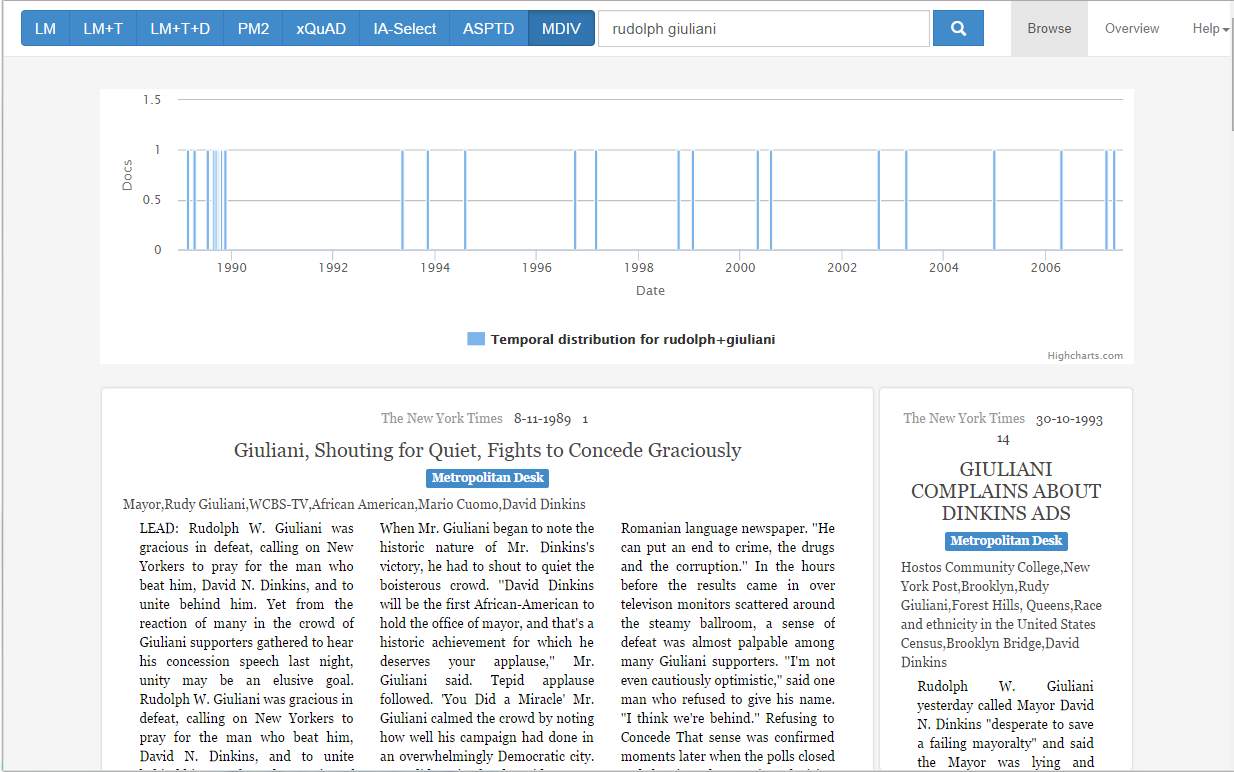
\includegraphics[width=0.9\columnwidth]{images/ui.png}
\caption{Newspaper interface with timeline.}
\label{fig:ui}
\end{figure}

The system was deployed on a live server. The same system also consists of the test collection evaluation setup; both the pooling logic and the interface.

\begin{itemize}
	\item URL: \texttt{http://pharos.l3s.uni-hannover.de:7080/ArchiveSearch/starterkit/}
	\item Evaluation: \texttt{http://pharos.l3s.uni-hannover.de:7080/ArchiveSearch/starterkit/relevance.html}
\end{itemize}

% subsection client_side (end)
% section architecture (end)
% chapter the_historical_search_system (end)